\documentclass[a4paper,12pt]{article}

\usepackage{fancyhdr}
\usepackage{lastpage}
\usepackage{amsmath}
\usepackage{tikz}
\usepackage{amsfonts}
\usepackage{csvsimple}
\usepackage{graphicx}


\newcommand{\V}[1]{\ensuremath{\vec{#1}}}
\newcommand{\F}[2]{\ensuremath{\frac{#1}{#2}}}
\newcommand{\Q}[1]{\newpage \section*{#1}}
\newcommand{\acc}[1]{\overset{..}{#1}}
\newcommand{\vel}[1]{\overset{.}{#1}}
\newcommand{\prt}[2]{\frac{\partial#1}{\partial#2}}
\newcommand{\LP}{\left(}
\newcommand{\RP}{\right)}

\pagestyle{fancy}
\lhead{Samuel Loomis}
\setlength{\headheight}{15pt}
\chead{Potential Energy Lab}
\rhead{\thepage\ of \pageref{LastPage}}
\lfoot{}
\cfoot{}
\rfoot{}

\begin{document}
\section*{Abstract}
\section*{Introduction}
\section*{Experiment}
\section*{Results}
Calculated results. (raw data and calculated values in back)\\
\csvautotabular{Force_Potential.csv}
\begin{figure}[h]
\centering
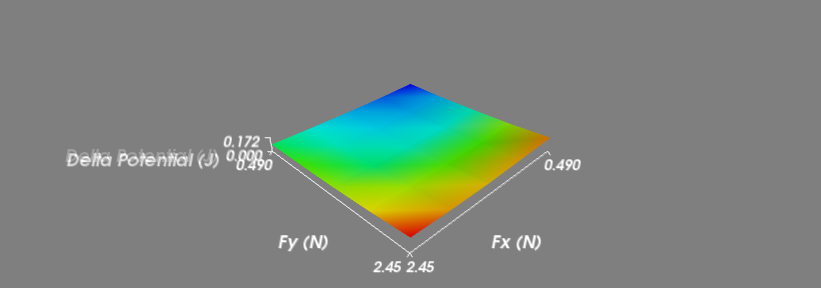
\includegraphics[width=5in]{ortho.png}
\caption{Orthoscopic view of the $\Delta$Potential energy. (Blue: low, Red: High)}
\end{figure}
\begin{figure}[h]
\centering
\includegraphics[width=5in]{sideview.png}
\caption{Side View}
\end{figure}
\section*{Conclusion}
\end{document}